\section{Experimental Results}


\begin{table}
\caption{Properties of the outer valence spectra of mixed ArXe clusters. Spectra of pure Ar and Xe clusters are included for reference. All spectra were recorded at $h\nu = 17$~eV, except for the pure Xe clusters ($h\nu = 60$~eV). Binding energies $E_b$ were determined as the centre of gravity of the respective feature, while band width $w$ are the FWHM of a Gaussian fit. The experimental Xe content of the clusters always is higher than in the original gas mixture (see Tab.\ \protect\ref{tab:cluster}). It was determined from the areas of the respective photolines, corrected by the respective atomic photoionization cross sections (Ar 33.0 Mb, Xe 51.3 Mb)\cite{samson2002}. Uncertainties are estimated as 3\,\% for the Xe content and 0.05~eV for the binding energies. Labels given in the first column refer to the expansion parameters in Tab.\ \protect\ref{tab:cluster}. $E_b$ and $w$ are in eV, $A$ is in \%. The binding energies can be compared to atomic values of 15.82~eV, 13.43~eV and 12.13~eV for Ar 3p and Xe 5p.
\label{tab:valence} }
\begin{tabular}{ l c c c c c c}
%
\toprule
  label & $E_b$(Ar 3p) & $w$(Ar 3p) & $E_b$(Xe 5p$_{1/2}$) &  $E_b$(Xe 5p$_{3/2}$) & $w$(Xe 5p$_{3/2}$)  &  $A$(Xe) \\
%
\midrule
% Ar, from Marko
 Ar (1) &  15.3  &  1.1 & & & &  \\
% Ar, from Marko 
 Ar (2) &  15.1  &  1.3 & & & &  \\
%
%  columns in the following: energies c.g. 51-plt-oval, widths Marko Diss., Xe content Marko Diss
% 1103 676, 679
 (a) & 15.36 & 0.9 & 13.07 & 11.75 & 0.85 & 12\\
% 1103 670
 (b) & 15.30 & 1.0 & 12.97 & 11.61 & 0.85 & 11\\
% 1103 671
 (c) & 15.25 & 1.1 & 12.91 & 11.52 & 1.08 & 10\\
% 1103 663
 (d) & 15.39 & 0.8 & 13.06 & 11.68 & 1.02 & 29\\
% 1103 640
 (e) & 15.31 & 0.6 & 12.96 & 11.44 & 1.24 & 53\\
% 0506 
Xe (1) & & & 12.76 & 11.19 & 1.18 & 100\\
%
\midrule
%
%  1004  886  (UHe, c.g. + roi values)
 886 & 15.15 & 1.3 & 12.59 & 11.01 & 1.24 & 19\\
\bottomrule
\end{tabular}
\end{table}


\begin{figure}[ht]
 \centering
 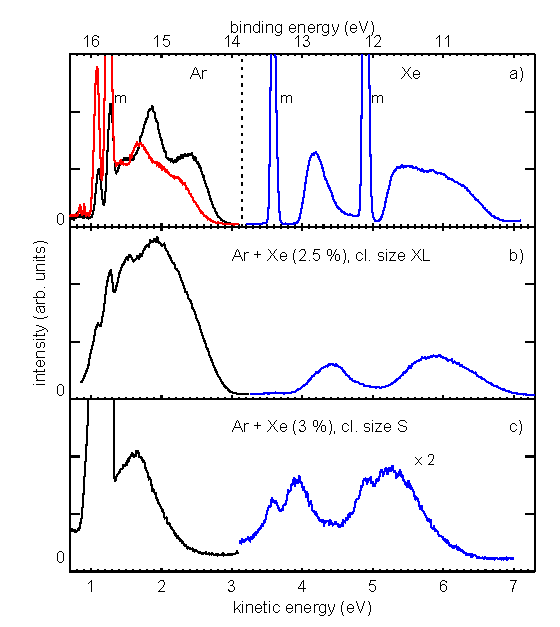
\includegraphics[width=8.5cm]{pics/figure_oval_1.pdf}
 \caption{
Outer valence photoelectron spectra of mixed Ar-Xe clusters, in comparison to the pure species. Panel a) shows the outer valence region of homogeneous Ar and Xe clusters, respectively (see text for details). The two lower panels show the spectra of the mixed species of different size. Sharp lines marked `m' result from photoionization of uncondensed atoms into the Ar 3p$_{1/2,3/2}$ and Xe 5p$_{1/2,3/2}$ final states. Labels in panels b) and c) give the Xe content in the expanding gas mixture, which is lower then the Xe content observed in the heterogeneous clusters. The photon energy used was 17~eV, apart from the pure Xe cluster spectrum (60 eV).
}
 \label{figure:oval1}
\end{figure}


\begin{figure}[ht]
 \centering
 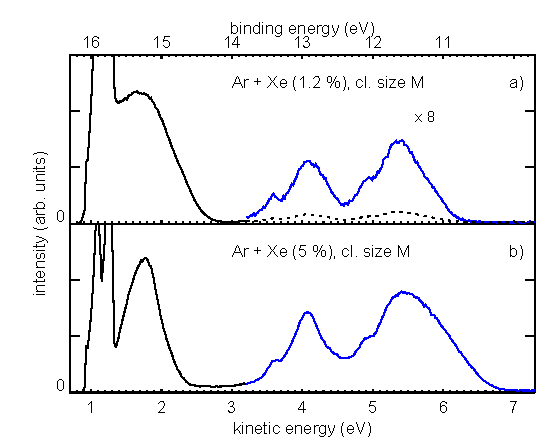
\includegraphics[width=8.5cm]{pics/figure_oval_2.pdf}
 \caption{
Outer valence photoelectron spectra of mixed Ar-Xe clusters from gas mixtures with different Xe concentration. See Fig.\ \ref{figure:oval1} and text for details.
}
 \label{figure:oval2}
\end{figure}



\begin{figure}[ht]
 \centering
 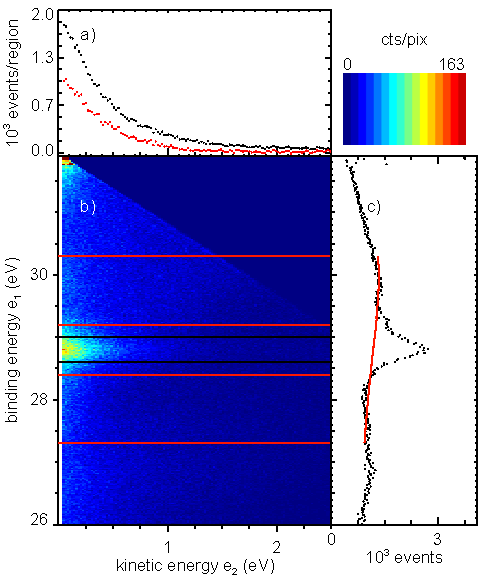
\includegraphics[width=8.5cm]{pics/figure_map.pdf}
 \caption{
Photon excited electron-electron coincidence spectrum of mixed Ar-Xe clusters in the inner valence region. Panel b): Color-coded map of coincident electron pairs, with the electron of higher kinetic named $e_1$. The energy of $e_1$ is given as binding energy, using the photon energy of $h\nu = 32$~eV. Panel c): Energy spectrum of primary electrons $e_1$, irrespective of the energy of the secondary electron (summation of the coincidence map along horizontal lines). The peak at a binding energy of 28.7~eV pertains to the Ar 3s photoelectron line.  Panel a): Energy spectrum of all secondary (ICD or ETMD) electrons $e_2$ pertaining to the Ar 3s binding energy region marked by two black bars. See text for details. Intensity is expressed as coincident events/pixel of 20~meV$^2$ (b) or as coincident events per interval of 20~meV (a,c). The color scale of panel b) is linear.
}
 \label{figure:map}
\end{figure}


\begin{figure}[ht]
 \centering
 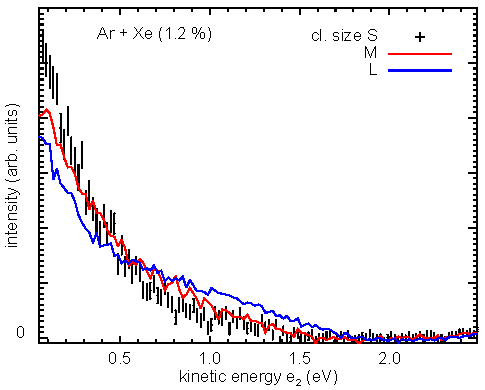
\includegraphics[width=8.5cm]{pics/figure_icd_12.pdf}
 \caption{
Energy spectrum of all coincident secondary (ICD or ETMD) electrons $e_2$ pertaining to primary electrons $e_1$ in the Ar 3s binding energy region. Spectra were recorded with a photon energy of $h\nu = 32$~eV. Black symbols with error bars show the data points for the smallest clusters measured (`S'), two larger clusters sizes are shown by the red and blue traces. For comparison, all spectra are shown area-normalized. 
}
 \label{figure:icd_12}
\end{figure}


\begin{figure}[ht]
 \centering
 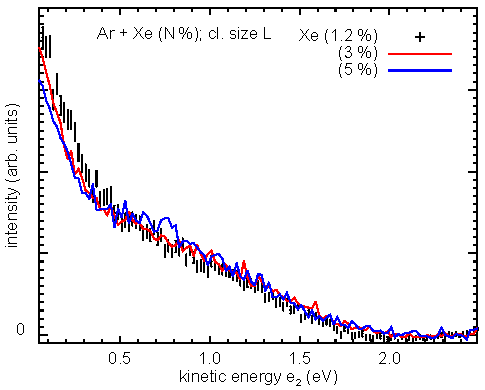
\includegraphics[width=8.5cm]{pics/figure_icd_l.pdf}
 \caption{
Energy spectrum of all coincident secondary (ICD or ETMD) electrons $e_2$ for clusters of the same size, but from gas mixtures with different Xe concentration. See Figure \protect\ref{figure:icd_12} for details.
}
 \label{figure:icd_l}
\end{figure}


\begin{figure}[ht]
 \centering
 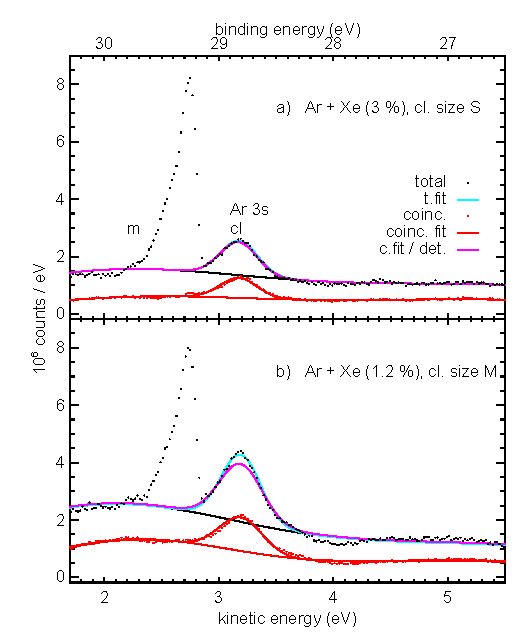
\includegraphics[width=8.5cm]{pics/figure_ival.pdf}
 \caption{
Photon excited electron spectra and electron-electron coincidence spectra of mixed Ar-Xe clusters in the inner valence region. Spectra show the Ar 3s photoline from clusters (`cl') and uncondensed Ar monomers (`m'), atop of a background resulting from inelastic intracluster scattering of outer valence photoelectrons.\protect\cite{hergenhahn2002} Black symbols: sum of non-coincident and coincident (1st hit) events, red symbols: coincident events only. Solid, colored lines show the results of various least-squares fits, see text for details.
}
 \label{figure:ival}
\end{figure}



\begin{figure}[ht]
 \centering
 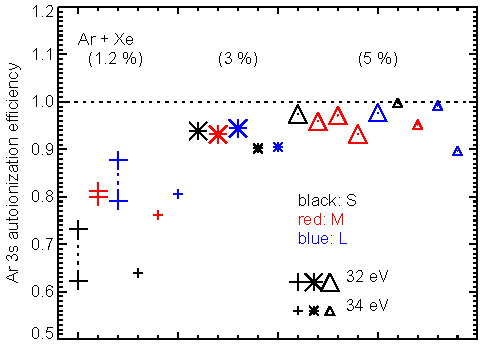
\includegraphics[width=8.5cm]{pics/figure_eff.pdf}
 \caption{
Efficiency of the decay of Ar 3s ionized states in ArXe clusters by emission of a secondary electron via ICD or ETMD. Values are arranged by Xe content of the initial gas mixture ('+' symbols: 1.2\,\%, asterisk: 3\,\%, triangle: 5\,\%). Symbol sizes indicate the photon energy (large symbols: 32 eV, small: 34 eV), and color indicates the cluster size (black symbols: S, red: M, blue: L). See text for details.
}
 \label{figure:eff}
\end{figure}
